\chapter{Results}

\shorthandoff{-} 

\section{Cloned \tax{promoter::GFP} sequences}
As most of the strains listed in the Table \ref{strains} were prepared several years ago and not by myself, we wanted to check which parts of the promoters we actually have cloned upstream of GFP gene in those cells.
For this purpose I designed pUA66\textunderscore insert primers (Table \ref{pcr}) based on the pUA66 and pU139 vector sequences (\hyperlink{pUA66seq}{Appendix 1} and \hyperlink{pUA66seq}{Appendix 2}).
PCR products were sequenced by Macrogen, Korea using Sanger platform.

\subsection{\tax{placZ::GFP} strains}
In the Fig. \ref{placZ} we can see that SC1\textunderscore D9 and MG1655 differ in \tax{lacZ} promoter region by a single SNP at position 39 nt upstream from \tax{lacZ} gene start codon (position 199 in Fig. \ref{placZ}).
These 2 strains have 3 more SNPs further downstream in \tax{lacZ} gene itself 
(positions 306, 324 and 363 in Fig. \ref{placZ}).
Based on the alignment of acquired \tax{lacZ} promoters sequences (Fig. \ref{placZ}) we can confirm that those assumed to originate from SC1\textunderscore D9 have an appropriate sequence as well as for MG1655.
\begin{figure}[ht]
  \centering
  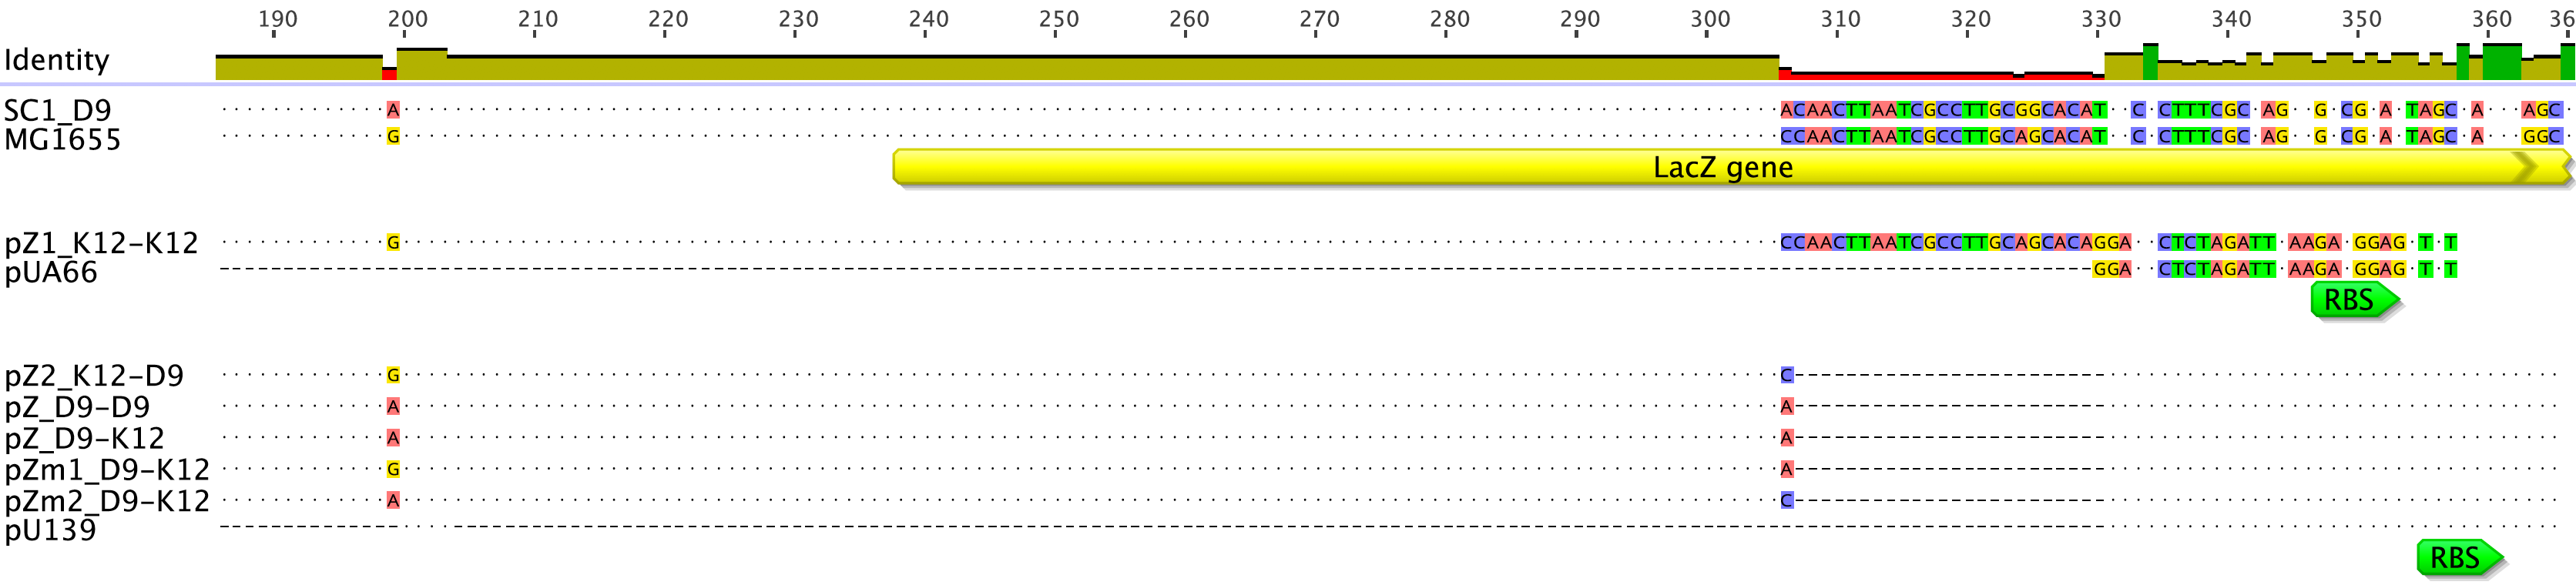
\includegraphics[scale=0.25]{text/Pictures/placZsequences.png}
	\caption{Excerpt of \tax{lacZ} promoters alignment with vectors and references. SC1\textunderscore D9 and MG1655 are reference sequences of \tax{lacZ} promoters from particular strains. pUA66 and pU139 are vectors aligned with no promoter upstream of GFP gene (not shown).}
	\label{placZ}
\end{figure}
Beside the SNPs in \tax{lacZ} promoter, the first SNP from \tax{lacZ} coding sequence is included in all vectors upstream of GFP.
Most of the strains possess pU139 as the vector except for pZ1\textunderscore K12-K12 which was acquired from Alon library \cite{zaslaver2006comprehensive}.
This strain have also longer part of \tax{lacZ} gene cloned into its pUA66 vector, potentially covering second SNP in it when compared to SC1\textunderscore D9.
This is not the only difference of pZ1\textunderscore K12-K12, as part of the \tax{lacI} gene is incorporated in all sequences listed in Fig. \ref{placZ} on the opposite site of the promoter (\hyperlink{placZalign}{Appendix 3}) and pZ1\textunderscore K12-K12 has this \tax{lacI} sequence almost 60 bp shorter than the rest of these strains.
Note, that strain pZ1m1\textunderscore D9-K12 and pZ1m2\textunderscore D9-K12 possess a recurrent mutation of the SNP in \tax{lacZ} promoter or \tax{lacZ} gene, respectively (from SC1\textunderscore D9 back to MG1655).
%%% I SUPPOSE IT'S POSSIBLE TO SAY THE SEQUENCE ABOVE IN A BETTER WAY, BUT I COULD FIND IT...
You can also realize that strain pZ2\textunderscore K12-K12 is not included in the Fig. \ref{placZ}.
The reason is that it was made by transforming the plasmid from pZ2\textunderscore K12-D9 into MG1655 after receiving the sequencing data and was not sequenced afterwards.

\subsection{\tax{precA::GFP} strains}
Both pA\textunderscore K12-K12 and pA\textunderscore K12-D9 strains have the same plasmid (pU139) as the latter was made by transforming plasmid from the former.
It was also confirmed by sequencing as well as that the sequence upstream of GFP gene correspond to \tax{recA} promoter of MG1655 (\hyperlink{precAalign}{Appendix 4}).
Similar to the cloned \tax{lacI}-\tax{lacZ} intergenic regions mentioned above, the sequence incorporated into pU139 and then transformed into these \tax{precA::GFP} strains includes parts of \tax{recA} gene downstream and \tax{pncC} gene upstream of the very promoter.


\section{Variation in promoter activity}
To explore the differences in promoter activity and genetic backgrounds, 4 h cultures grown in M9 minimal media with a single carbon source were assayed using flow cytometry (see Materials and Methods).
Exported FCS files were then analysed in R - used scripts are available at \href{https://github.com/marketavlkova/}{GitHub} repositories.

\subsection{Activity of \tax{lacZ} promoters}



% 17.9.2018
% where is this name from?
\section{Construction of pADOUCH plasmid}
As we could see, \tax{lacZ} promoters cloned into plasmids were active even in non-lactose environments, but that is not the case for strain ASC662 which has GFP gene integrated into chromosome.
We hypothesise, that this differential results might be caused by the naturally low amounts of LacI repressor present in a cell.
When a cell makes multiple copies of \tax{lacZ} promoter by its sequence on a plasmid, all LacI proteins become saturated and a part of the promoters escape the repression, even though the plasmids used should produce only several copies within a cell \cite{zaslaver2006comprehensive}.
To confirm that we decided to place the \tax{placZ::GFP} sequences into chromosome, creating only one additional \tax{lacZ} promoter per a cell.

We have available pLW001 plasmid which is suitable for chromosomal integration (\hyperlink{pLW001}{Appendix 5}) however, this plasmid lacks ribosome binding site (RBS).
Thus we constructed a new plasmid by replacing the GFP gene present in pLW001 vector with the GFP sequence we have in our negative control plasmid pUA66 (\hyperlink{pUA66seq}{Appendix 1}) together with its strong RBS, some additional restriction sites and a transcriptional terminator (Fig. \ref{cloning}).
\begin{figure}[h!]
  \centering
  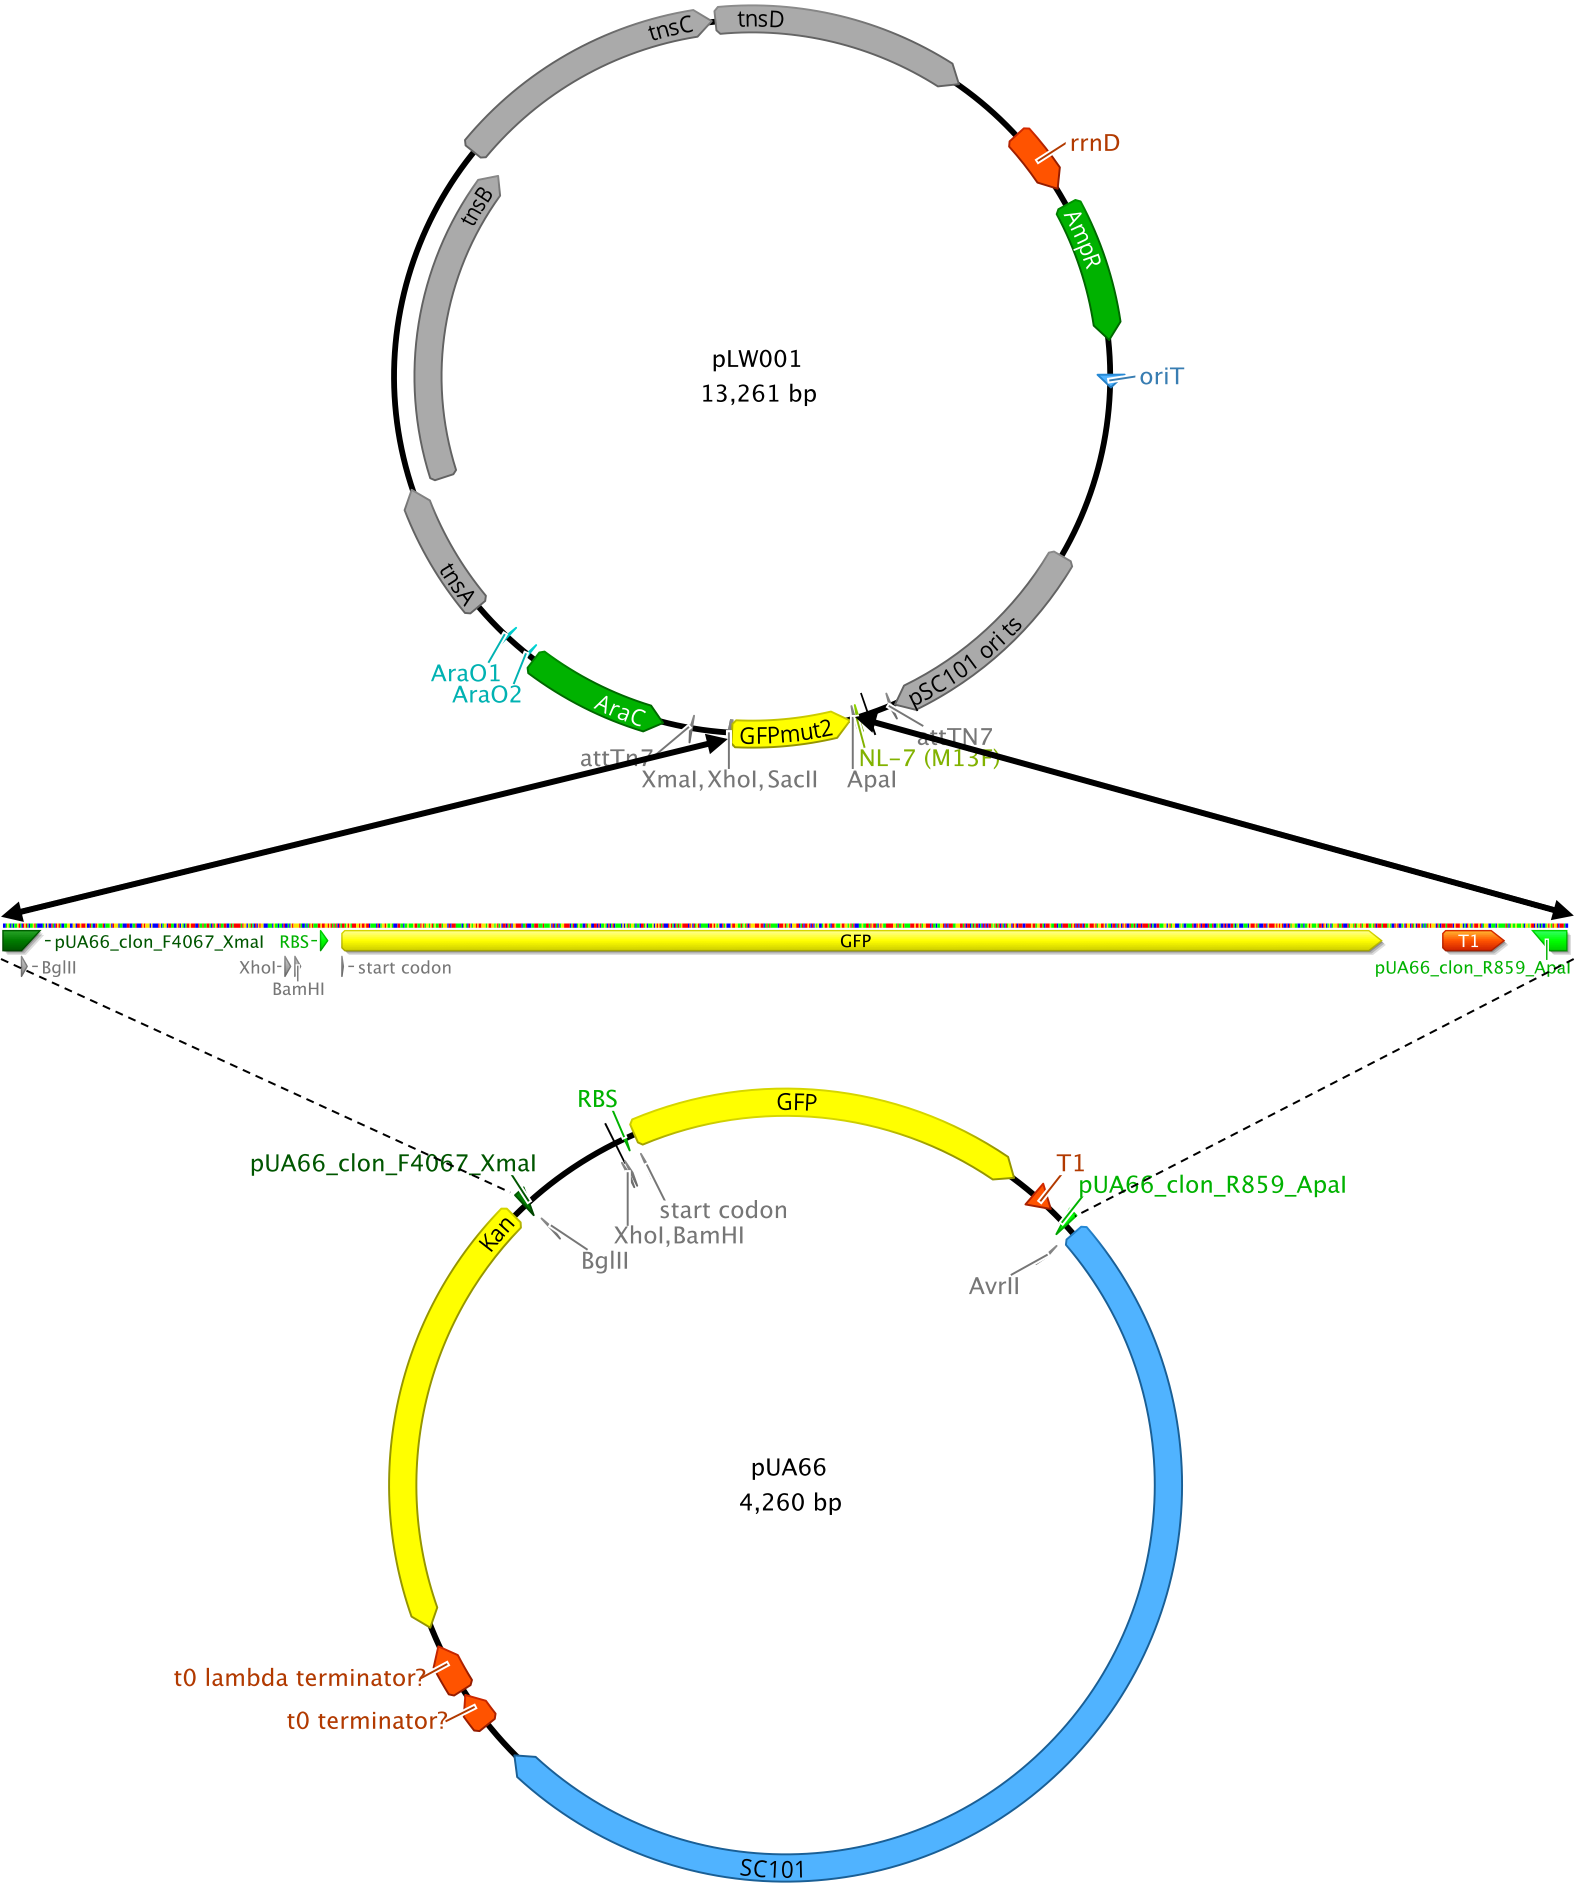
\includegraphics[scale=0.4]{text/Pictures/Cloning.png}
	\caption{Scheme of pADOUCH plasmid construction by replacing GFP sequence from pLW001 vector by sequence from pUA66 plasmid.}
	\label{cloning}
\end{figure}

% 17.9.2018
% "tested" - showing what? e.g. "showing that successful integration had occurred."
We successfully amplified sequence of expected length (1.1 kb) in all 8 transformants tested (Fig. \ref{colonyPCR}).
\begin{figure}[h!]
  \centering
  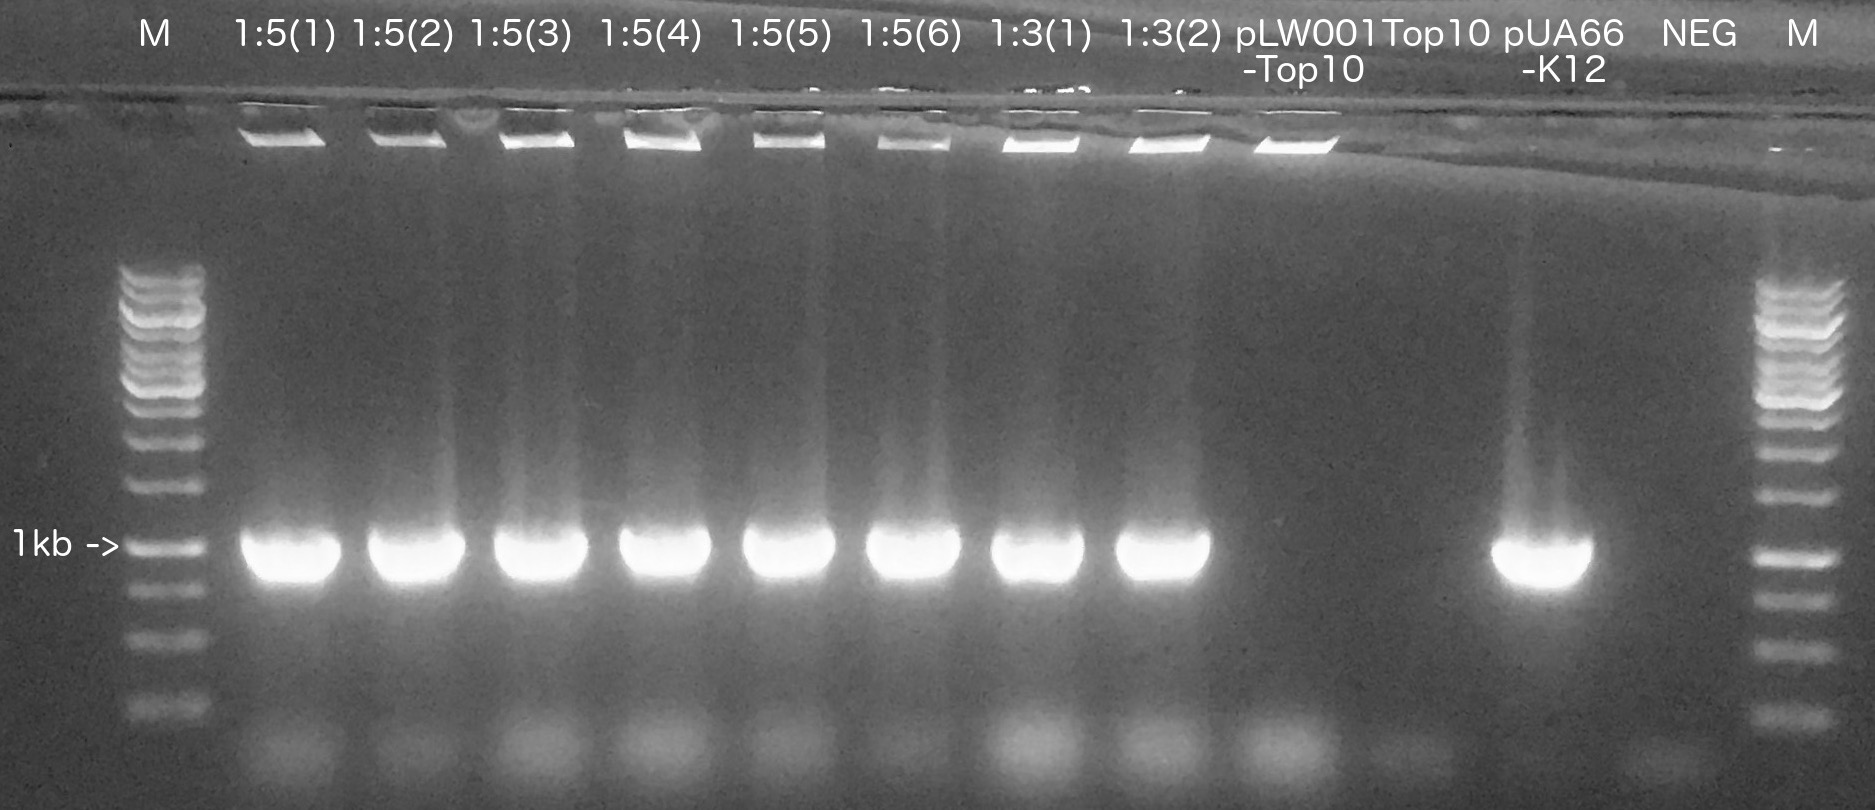
\includegraphics[scale=0.2]{text/Pictures/ColonyPCR.jpg}
	\caption{Electrophoresis of colony PCR using pUA66\textunderscore clon primers; M - marker; first 8 samples (1:5(1) - 1:3(2)) - tested clones; pLW001-Top10 and Top10 - negative controls with template DNA; pUA66-K12 - positive control; NEG - negative control without template DNA.}
	\label{colonyPCR}
\end{figure}
Sanger sequencing confirmed the presence of desired insert in digested pLW001 vector.
However, we identified four SNPs compared to the expected sequence in GFP gene (Fig. \ref{1:3(1)seq}).
But as both sequenced clones have exactly the same SNPs (\hyperlink{pADOUCHseq}{Appendix 6}) and all of these SNPs are synonymous (Fig. \ref{1:3(1)seq}), we inferred that the reference sequence of GFP gene in the pUA66 plasmid was inaccurate.
Complete revised sequence of pADOUCH vector can be found in \hyperlink{pADOUCHwhole}{Appendix 7}.
\begin{figure}[ht]
  \centering
  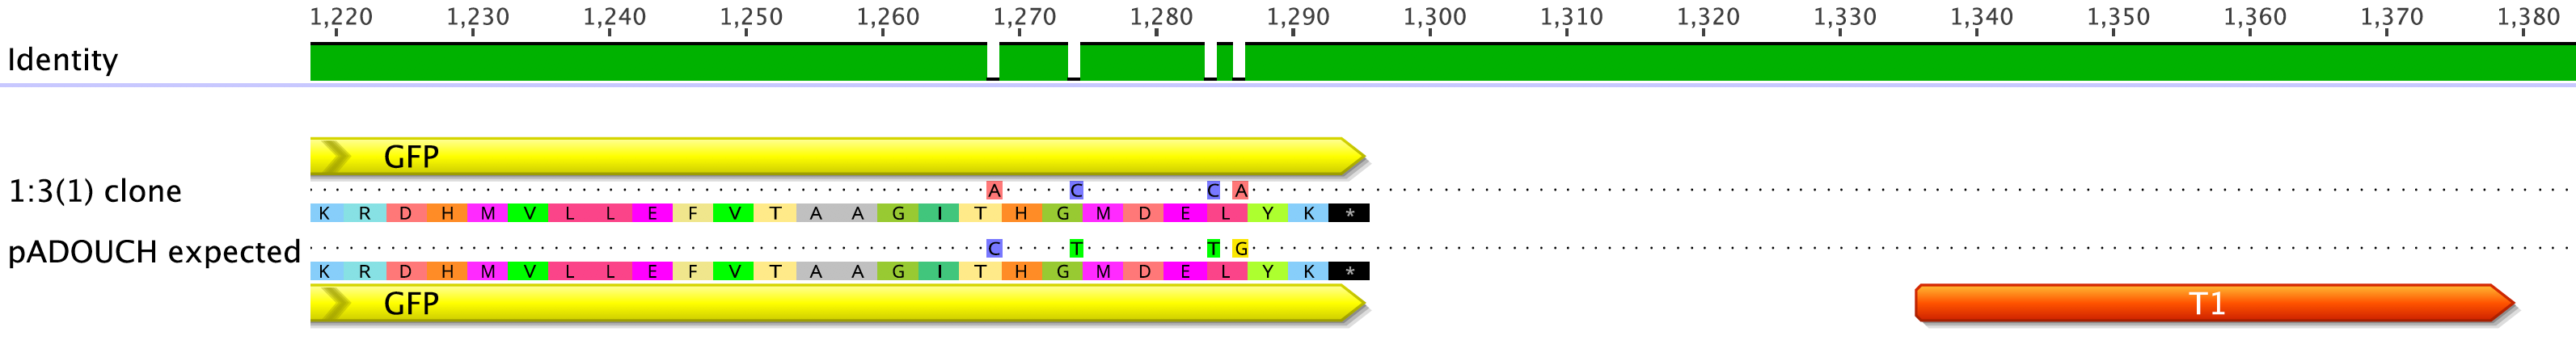
\includegraphics[scale=0.26]{text/Pictures/pADOUCHseq.png}
	\caption{Excerpt of 1:3(1) clone sequence alignment with expected pADOUCH references. DNA sequence is dotted except for SNPs; protein sequence is always beneath its DNA sequence.}
	\label{1:3(1)seq}
\end{figure}

\shorthandon{-} 
%%%%%%%%%%%%%%%%%%%%%%%%%%%%%%%%%%%%


